\documentclass[tikz]{standalone}
\usepackage{tikz}

\begin{document}
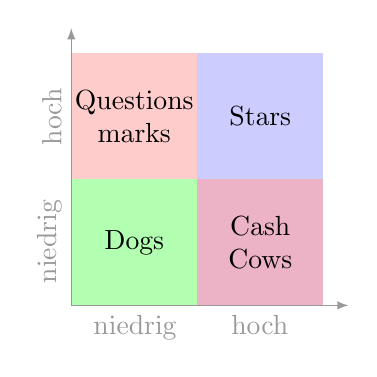
\begin{tikzpicture}[scale=1.6]

\fill[red!20] (0,2)rectangle++(1,-1)node[midway, black, align=center]{Questions \\ marks};
\fill[blue!20] (1,2)rectangle++(1,-1)node[midway, black, align=center]{Stars};
\fill[green!30] (0,1)rectangle++(1,-1)node[midway, black, align=center]{Dogs};
\fill[purple!30] (1,1)rectangle++(1,-1)node[midway, black, align=center]{Cash \\ Cows};

\draw[-latex, black!40] (0,0)--++(0,2.2)node[pos=.23, sloped, above]{niedrig}node[pos=.68, sloped, above]{hoch};
\draw[-latex, black!40] (0,0)--++(2.2,0)node[pos=.23, below]{niedrig}node[pos=.68, below]{hoch};






\end{tikzpicture}
\end{document}